\documentclass{article}

\usepackage{amsmath,amssymb,graphicx,geometry,enumitem,caption,subcaption}
\usepackage{xepersian}

\newcounter{qnumber}
\setcounter{qnumber}{1}

\newcommand{\Q}{
\textbf{سوال \theqnumber)}
\stepcounter{qnumber}
}

\setlength{\parindent}{0mm}
\setlength{\parskip}{3mm}
\settextfont{XB Niloofar}

\begin{document}

\begin{center}
\large

به نام او

آزمون پایان ترم سیگنال ها و سیستم ها
\end{center}

\hrulefill

\large


برای سیگنال پیوسته‌ی
$
x(t)
$
با تبدیل فوریه‌ی زیر،

\begin{center}
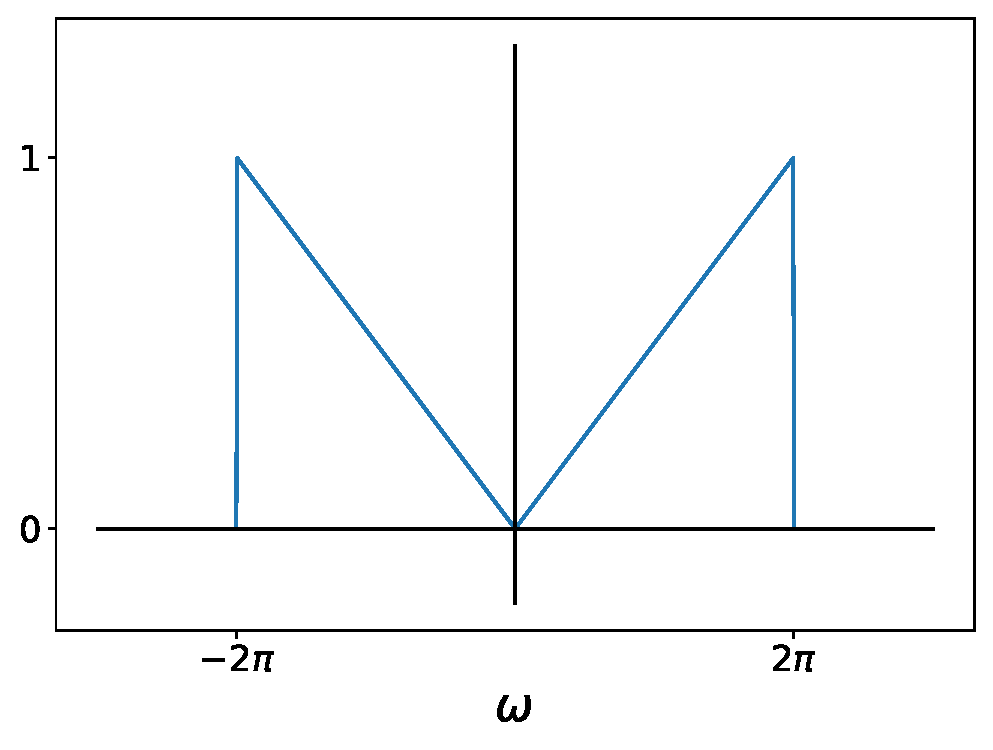
\includegraphics[width=63mm]{X(jw).eps}
\end{center}

(محور افقی، نشان دهنده‌ی فرکانس زاویه ای $\omega$ است.)

الف) مقدار نرخ نایکوئیست را تعیین کنید و آن را با $F_s$ نشان دهید. سپس طیف سیگنال نمونه برداری شده با نرخ $2F_s$ را رسم کنید.

ب) فرض کنید سیگنال $x(t)$ را با نرخ 
$
\frac{3F_s}{4}
$
نمونه برداری کرده و آن را 
$
\hat x[n]
$
نامیده ایم. به عبارت دیگر
$$
\hat x[n]=x(\frac{t}{3F_s/4})
$$

اگر با بهره گیری از نمونه های 
$
\hat x[n]
$
، سیگنال پیوسته‌ی $y(t)$ را با نرخ نمونه برداری 
$
\frac{3F_s}{4}
$
بسازیم، آیا 
$
x(t)
$
با 
$
y(t)
$
برابر است؟

ج) (امتیازی) جزئیات ریاضی محاسبه‌ی $y(t)$ را انجام دهید.

% سیگنال پیوسته‌ی $y(t)$ را به گونه ای بیابید که دارای دو خاصیت زیر باشد
%$$
%|Y(j\omega)|=0\quad,\quad |\omega|>\pi \frac{F_s}{2}
%$$
%$$
%\hat y[n]=y(\frac{t}{F_s/2})=\hat x[n]
%$$


\end{document}